\subsection{NMF applied to the Daya Bay matrix}
The separable NMF algorithm we implemented fits nicely into a data parallel programming model. After the initial distributed TSQR the remainder of the algorithm is computed serially on the driver. The Daya Bay matrix is especially amenable to this approach, as the extreme aspect ratio of the data set implies that the TSQR is particularly efficient.

\paragraph{C+MPI vs. Spark.}

\begin{figure*}[thb!]
\begin{center}
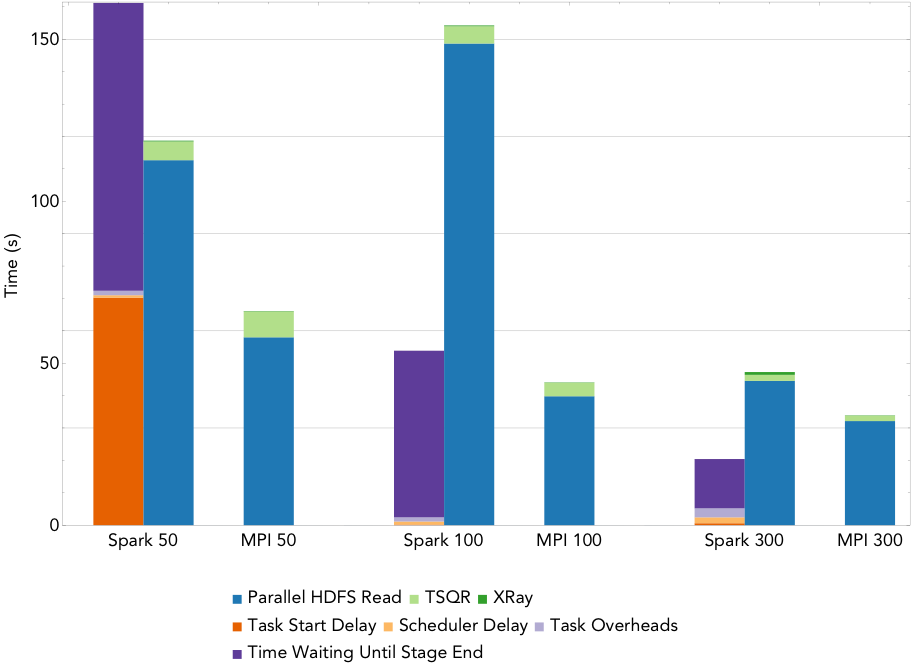
\includegraphics[width=.9\textwidth]{fig/nmf_run_times.png}
\caption{Running time breakdown when using NMF to compute a rank 10 approximation to the 1.6TB Daya Bay matrix at 
  node counts of 50, 100, and 300. Each bin depicts the sum, over all stages, of the time spent in that bin by the average task within a stage.}
\label{fig:nmfrt}
\end{center}
\end{figure*}

The TSQR algorithm used performs a single round of communication using a flat binary tree. Because there are few columns, the NMF algorithm is entirely I/O-bound. Figure~\ref{fig:nmfrt} gives the running time breakdown when computing rank 10 approximations using the MPI implementation of NMF on 50 nodes, 100 nodes, and 300 nodes. 
Each bin represents the sum, over all stages, of the time spent in that bin by the average task within a stage.

The running time for NMF is overwhelmingly dominated by reading the input. In comparison, TSQR and~\textsc{XRay} have negligible running times. Figure~\ref{fig:nmfrt} shows that the HDF5 read time does not scale linearly with the number of nodes and is the primary source of inefficiency -- this is due to saturating the system bandwidth for 72 OSTs. \textsc{XRay}, which is computed on the driver, is a sequential bottleneck and costs ~$100$ms at all node counts. TSQR only improves by tens of milliseconds, costing $501$ms, $419$ms, and $378$ms on 50, 100, and 300 nodes, respectively. This poor scaling can be attributed to hitting a communication bottleneck. Forming the TSQR binary tree is expensive for small matrices, especially using flat MPI. We did not tune our TSQR reduction tree shapes or consider other algorithms since TSQR is not the limiting factor to scalabilty. These results illustrate the importance of I/O scalability when performing terabyte-scale data parallel analytics on a high-performance architecture using MPI.

Figure~\ref{fig:nmfrt} also illustrates the running time breakdown for the Spark implementation of NMF on 50, 100, and 300 nodes. Unlike the MPI implementation, the Spark implementation incurs significant overheads due to task scheduling, task start delays, and idle time caused by Spark stragglers. For the 50 node run we configured Spark to use double the number of partitions as physical cores because we encountered out-of-memory errors using fewer partitions--- this incurs a task start delay overhead because some only half of the total tasks can be executed concurrently. The number of partitions was not doubled for the 100 and 300 node runs, so the task start delay overhead is much smaller for these runs. Similar to the MPI results, most of the running time is spent in I/O and Spark overheads, with a small amount of time spent in TSQR and \textsc{XRay}. Figure~\ref{fig:nmfrt} shows that the Spark implementation exhibits good strong scaling behavior up to 300 nodes.  Although the NMF algorithm used is entirely data parallel and suitable for Spark, we observed a $4\times$, $4.6\times$, and $2.3\times$ performance gap on 50, 100, and 300 nodes, respectively, between Spark and MPI.

\begin{figure}[h]
\centering
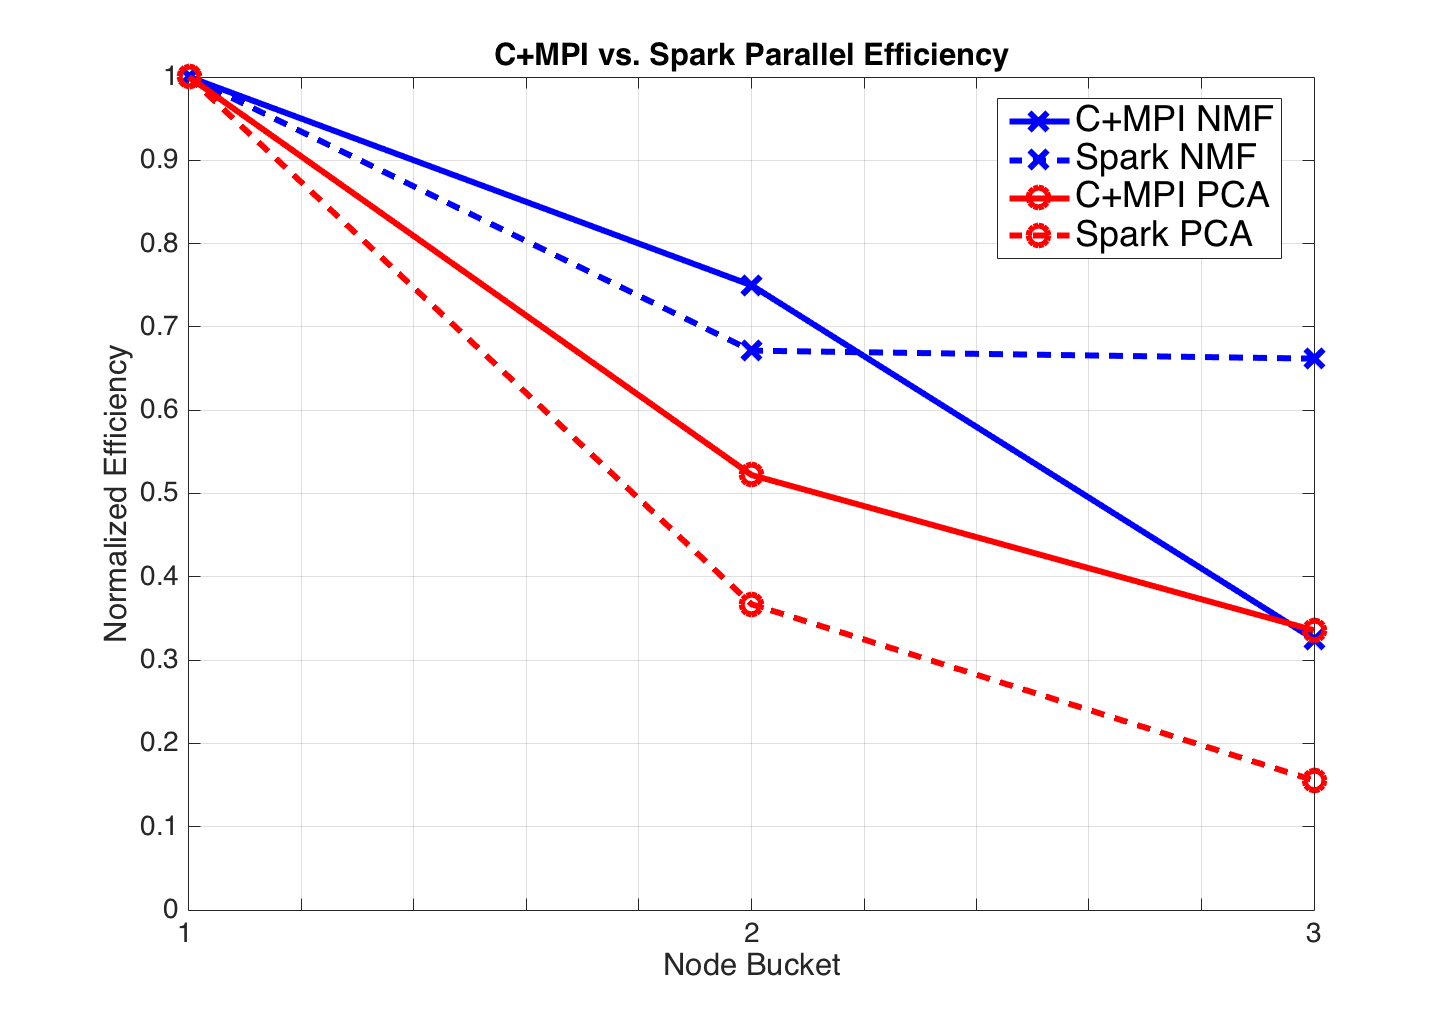
\includegraphics[width=.9\textwidth]{fig/peff.png}
\caption{Comparison of parallel efficiency for C+MPI and Spark. The x-axis label ``Node Bucket'' refers to the node counts. For NMF these are 50, 100, and 300 nodes (left to right) and 100, 300, and 500 nodes for PCA. For both algorithms, efficiency is measured relatively to the performance at the smallest node count.}
\label{fig:peff}
\end{figure}

Figure~\ref{fig:peff} shows the parallel efficiencies of the MPI and Spark implementations of NMF, normalized to the 50 node running time of the respective parallel frameworks. MPI NMF is completely dominated by I/O and the results are primarily indicative of scaling issues in the I/O subsystem. Spark NMF displays good scaling with more nodes; this is reflected in the parallel efficiency. However, the scaling is due primarily to decreases in the Spark overhead.

\paragraph{Science Implications.}
We are currently investigating the results of the NMF decomposition. Preliminary analysis indicates that we will need to augment the input data with non-linear features to make the input signals invariant to rotations and translations. Our eventual goal is to learn event-specific classifiers from the loadings of the NMF basis vectors. The classification will enable us to accomplish the final goal of segmenting and classifying the timeseries of sensor measurements. While implementing and verifying the scientific value of the entire pipeline is out of scope for this report, we have demonstrated the ability to apply our Spark NMF implementation to the TB-sized Daya Bay matrix. Together with feature augmentation, this will enable us to explore more advanced methods in the near future.

\subsection{PCA applied to the climate matrices}

We compute the PCA using an iterative algorithm whose main kernel is a distributed matrix-vector product. Since matrix-vector products are data parallel, this algorithm fits nicely into the Spark model. Because of the iterative nature of the algorithm, we cache the data matrix in memory to avoid I/O at each iteration.

\begin{figure*}[th!]
\centering
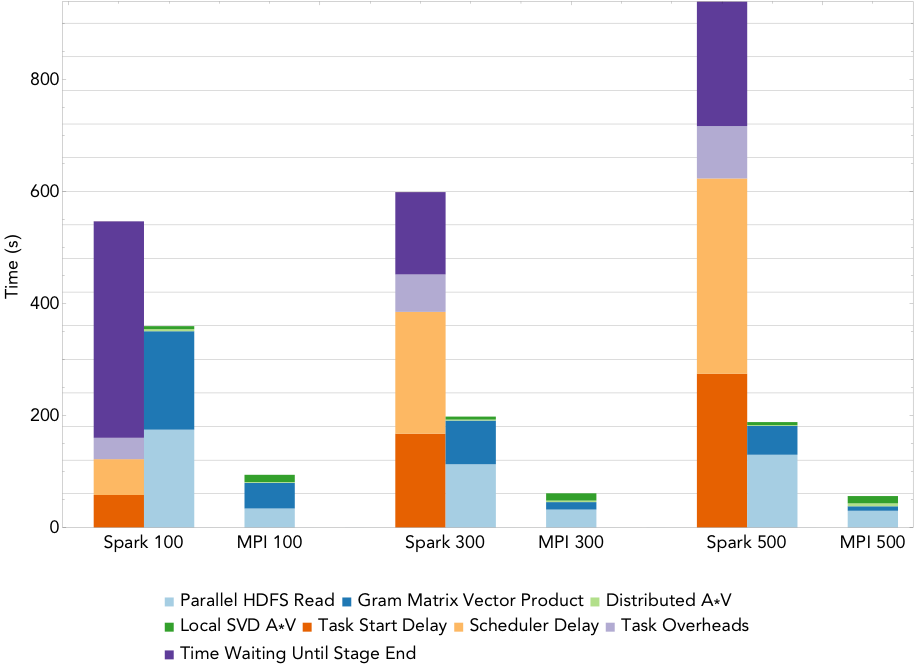
\includegraphics[width=.9\textwidth]{fig/ocean_pca_times.png}
\caption{Running time breakdown of PCA on the 2.2TB Ocean matrix at node counts of 100, 300 and 500. Each bin depicts the sum, over all stages, of the time spent in that bin by the average task within a stage.}
\label{fig:pcart}
\end{figure*}

\begin{figure}[th!]
\centering
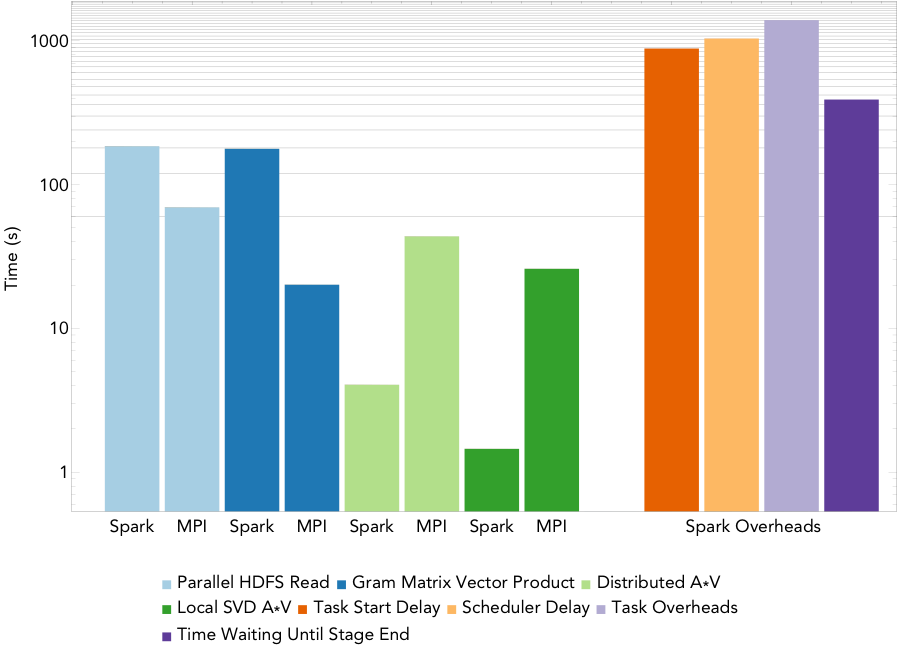
\includegraphics[width=.9\textwidth]{fig/hero_pca_times.png}
\caption{Running time comparison of the Spark and MPI implementations of PCA on the 16TB Atmosphere matrix. Each bin depicts the sum, over all stage, of the time spent in that bin by the average task within a stage.}
\label{fig:hero}
\end{figure}

\paragraph{C+MPI vs. Spark.}
Figure~\ref{fig:pcart} shows the running time breakdown results for computing a rank-20 PCA decomposition of the Ocean matrix on 100, 300, and 500 nodes using the MPI implementation. Each bin depicts the sum, over all stages, of the time spent in that bin by the average task within a stage.

I/O is a significant bottleneck and does not exhibit the scaling observed for NMF in Figure~\ref{fig:nmfrt}. The I/O time is reduced going from 100 to 300 nodes, but not 300 to 500 nodes because the I/O bandwidth is saturated for the stripe size and number of OSTs used for the Daya Bay and Ocean data sets. The Gram matrix-vector products are a significant portion of the running time but scale linearly with the number of nodes. The matrix-matrix product ($AV$) does not scale due to a communication bottleneck. The bottleneck is because we compute a rank-$20$ PCA which makes communicating $V$ expensive. This cost grows with the number processors since it is entirely latency dominated. The final SVD of $AV$ is a sequential bottleneck and does not scale. Unlike NMF the sequential bottleneck in PCA is significant; future implementations should perform this step in parallel.

Figure~\ref{fig:pcart} also shows the scaling and running time breakdown of the Spark PCA implementation for 100, 300, and 500 nodes. The Gram matrix-vector products scale linearly with the number of nodes, however this is outweighed by inefficiencies in Spark. At this scale, Spark is dominated by bottlenecks due to scheduler delays, task overhead and straggler delay times. Task overhead consists of deserializing a task, serializing a result and writing and reading shuffle data. The Spark scheduling delay and task overhead times scale with the number of nodes, due to the centralized scheduler used in Spark. The iterative nature of the PCA algorithm stresses the Spark scheduler since many tasks are launched during each iteration. Under this workload we observed a 10.2$\times$, 14.5$\times$, and 22$\times$ performance gap on 100, 300, and 500 nodes, respectively, between Spark and MPI. The disparity between the costs of the $AV$ products and sequential SVDs in MPI and Spark can be attributed to the use of single-threaded BLAS for MPI and multi-threaded BLAS for Spark.

Figure~\ref{fig:peff} shows the parallel efficiency of MPI PCA and Spark PCA. We observed that the MPI version hits an I/O bottleneck, a communication bottleneck in the $AV$ product and a sequential bottleneck in SVD($AV$). All of these are limiting factors and introduce inefficiencies to MPI PCA. Spark PCA is less efficient than MPI PCA due to scheduler delays, task overhead and straggler effects. The scheduler delays are more prominent in PCA than in NMF due to the larger number of tasks. NMF makes a single pass over the data whereas PCA makes many passes over the data and launches many tasks per iteration.

\paragraph{PCA Large-Scale Run.}
We used all 1600 Cori nodes to compute a rank-20 PCA decomposition of the 16TB Atmosphere matrix. In order to complete this computation in Spark in a reasonable amount of time, we fixed the number of iterations for the EVD of $A^TA$ to $70$ iterations. MPI PCA was able to complete this run in $160s$. Unfortunately we were unsuccessful at launching Spark on $1600$ nodes; after many attempts we reduced the number of nodes to $1522$. At this node count, Spark PCA successfully completed the run in $4175s$. Figure~\ref{fig:hero} shows the head-to-head running time comparison for this full-system run; each bin depicts the sum, over all stages, of the time spent within that bin by the average task within a stage. The Gram matrix-vector products are an order of magnitude more costly in Spark. We noticed that the tree-aggregates were very slow at full-system scale and are the likely cause of the slow Gram matrix-vector products. The $AV$ product and SVD are much faster in Spark than in MPI due to its use of multiple OpenBLAS threads. Finally, we observed that the Spark overheads were an order of magnitude larger than the communication and computation time.

\paragraph{Science Implications.}
For the 2.2TB Ocean data set, the first two temporal ``empirical orthogonal functions'' (EOFS)--- corresponding to right singular vectors--- fully capture the annual cycles. The remaining time series show abrupt changes due to the 1983 El Ni\~no Southern Oscillation (ENSO), and more significantly, the record-breaking ENSO of 1997--98. The intermediate modes contain a complex interplay of various timescales, which is currently under investigation. The spatial EOFs, corresponding to the left singular vectors, show the relative dominance of the Indian Ocean Dipole and the classic warm pool--cold tongue patterns of ENSO at various depths below the ocean surface. Because of the 3D nature of the EOFs, we are able to see that the dynamic near the thermocline is most dominant, rather than that closer to the surface. Further, there are several smaller scale features that have a strong influence at different depths. Work is on-going to understand the nature of these different spatial patterns and the factors that influence their relative dominance.
 
\subsection{CX on the Mass-spec matrix}
\begin{table}[t]
\centering
\begin{tabular}{|c|c|c|c|} \hline
Algo & Size & \# Nodes & Spark Time (s)\\ \hline
\multirow{3}{*}{CX} & \multirow{3}{*}{1.1 TB} & $60$ & $1200$\\
{} & {} & $100$  & $784$\\
{} & {} & $300$ & $542$\\ \hline
\end{tabular}
\caption{Spark CX running times}
\label{tab:cxscale}
\end{table}
Much like PCA, the CX decomposition requires a parallel Gramian multiply, a distributed matrix-matrix product and a randomized SVD in order to compute extremal columns of $A$. CX is applied to the sparse 1.1TB MSI matrix, which is stored in the Parquet format. Table~\ref{tab:cxscale} shows the running times and scaling behavior of Spark CX. We found that Spark exhibited good scaling for the range of nodes tested and attained speedups of $1.5\times$ and $2.2\times$ on 100 and 300 nodes, respectively. The corresponding parallel efficiencies are 90\% for 100 nodes and 44\% for 300 nodes. These results show that the behavior of CX is similar to that of PCA, which is due to the overlap in their linear algebra kernels.

\paragraph{Science Interpretation.}
 The CX decomposition selected ions in three narrow regions of $m/z$. Among those ions identified as having significant leverage scores are ions at $m/z$ values of 439.0819, 423.0832, and 471.1276, which correspond to neutral losses of $\rm{CH_2}$, $\rm{CH_2O}$, and a neutral ``gain'' of $\rm{H_2O}$ from the 453.0983 ion.  These relationships indicate that this set of ions, all identified as having significant leverage scores, are chemically related.  That fact indicates that these ions may share a common biological origin, despite having distinct spatial distributions in the plant tissue.  

\subsection{Summary of Spark vs. C+MPI performance comparison}
We have demonstrated that matrix factorizations (which have traditionally been implemented using high-performance parallel libraries) can be implemented on Spark, and that Spark can run on large node counts on HPC platforms. By exploring the performance trade-offs of Spark matrix factorizations and comparing to traditional MPI implementations we have gained insights into the factors affecting Spark's scalability. Table~\ref{tab:matrix} summarizes the wall-clock times of the MPI and Spark implementations of the considered factorizations, and Table~\ref{tab:perfgaps} summarizes the performance gaps between Spark and MPI. These gaps range between $2\times - 25\times$ when I/O time is included in the comparison and $10\times - 40\times$ when I/O is not included. These gaps are large, but our experiments indicated that Spark I/O scaling is comparable to MPI I/O scaling, and that the computational time scales. The performance gaps are due primarily to scheduler delays, straggler effects, and task overhead times. If these bottlenecks can be alleviated, then Spark can close the performance gap and become a competitive, easy-to-use framework for data analytics on high-performance architectures.

\begin{table}[tbh]
\centering

\begin{tabular}{|c|c|c|c|c|c|} \hline
Algo & Size & \# Nodes & MPI Time (s) & Spark Time (s)\\ \hline
\multirow{3}{*}{NMF} & \multirow{3}{*}{1.6 TB} & $50$ & $66$ & $278$\\
{} & {} & $100$  & $45$ & $207$\\
{} & {} & $300$ & $30$ & $70$\\ \hline
\multirow{4}{*}{PCA} & \multirow{3}{*}{2.2 TB} & 100 & 94 & 934\\
 {} & {} & 300 & 60 & 827\\
 {} & {} & 500 & 56 & 1160\\ \cline{2-5}
 {} & {16 TB} & {MPI: 1600 Spark: 1522} & 160 & 4175 \\ \hline
\end{tabular}
\caption{{Summary of Spark and MPI running times.}}
\label{tab:matrix}
\end{table}

\begin{table}[tbh]
\begin{center}
\begin{tabular}{|c|c|c|c|} \hline
Algo & \# Nodes & Gap with I/O & Gap without I/O\\ \hline
\multirow{3}{*}{NMF} & $50$ & $4\times$ & $21.2 \times$\\
{} & $100$  & $4.6\times$ & $14.9\times$\\
{} & $300$ & $2.3\times$ & $15.7\times$\\ \hline
\multirow{4}{*}{PCA} & 100 & $10.2\times$ & $12.6\times$\\
 {} & 300 & $14.5\times$ & $24.7\times$\\
 {} & 500 & $22\times$ & $39.3\times$\\ \cline{2-4}
 {} & {MPI: 1600 Spark: 1522} & $26\times$ & $43.8\times$\\ \hline
\end{tabular}
\end{center}
\caption{Summary of the performance gap between the MPI and Spark implementations.}
\label{tab:perfgaps}
\end{table}

